\chapter{Towards a Probabilistic Approach}
\label{ch:ProbabilisticPOC}

My goal in \cref{part:generalModel} is to demonstrate how the initial predictive model given in \cref{ch:lockdown} can be further developed to form a practical and generalisable predictive soundscape model. So far, in \cref{ch:mlmann,ch:whostudy}, I have demonstrated the potential benefits of incorporating additional sound source information and secondary factors. At this point, after several years and studies working closely with the \gls{isd} data and the ISO 12913 specifications, it was important to further examine the analysis methods being used. Therefore, this chapter, originally published as \citet{Mitchell2022How}, interrogates the analysis methods presented in the ISO and further develops a new method of representing the soundscape of a space. Finally, I discuss how to bring the predictive model expanded throughout this thesis in line with the suggested improvements to the existing analysis and visualisation methods. 

\section{Summarising the soundscape assessment of a location}
The studies presented so far have generally followed the analysis methods presented in \citet{ISO12913Part3}. While the assessment methods available are able to record the soundscape perception of a single individual, and that person's perception is valid for themselves, it is not appropriate to then state that it is representative of the collective perception of that soundscape. In order to characterise the soundscape of a particular space or time, perceptual responses from multiple people must be collected and subsequently summarised or aggregated to describe the general soundscape of the location. The ISO guidelines stipulate a minimum of 20 participants for a soundwalk, with these broken up into sessions of no more than 5 participants at a time. Part 3 then provides the recommended methods for analysing this data.

Annex A.2 of ISO 12913 Part 3 provides the statistical measures to be used on the raw PA responses. The recommended measure of central tendency is the median, while the recommended measure of dispersion is the range. These are chosen as the data is ordinal by nature, however as will be demonstrated later, they have significant limitations. Although it is unclear, the implied intention is then that the median value of each PA is fed into \cref{eqn:pleasant,eqn:eventful} presented in \cref{chap:methods} to calculate the ISOPleasant and ISOEventful values, which can then be plotted in a two-dimensional scatter plot. Thus the standard suggests that (1) the projection method equations are not applied to individual responses and (2) only the median assessment of a location should be plotted.

\section{Limitations of the ISO}
How the \citet{ISO12913Part3} methods should be applied to represent the soundscape of a location has not been adequately discussed in previous literature, nor sufficiently in Part 3 of ISO 12913 itself. Indeed, in Section A.3, the technical specifications document state that \citep[p. 5]{ISO12913Part3}:

\begin{quote}
  Results can be reported in a two-dimensional scatter plot with coordinates for the two dimensions ‘pleasantness’ and ‘eventfulness’. The coordinates for ‘pleasantness’ are plotted on the X-axis, and the coordinates for ‘eventfulness’ on the Y-axis. Every data point in the scatter plot represents one investigated site.
\end{quote}

However, it is not made clear whether this single point on the circumplex can be considered to be a realistic representation of the average perception of the acoustic environment. This is how I have so far represented the soundscape of a location (as in \cref{fig:circumplex-locations,fig:circumplex-vectors}). Here, I will argue that this representation is incomplete. Effectively, there is no representation of dispersion in the soundscape assessment, nor a recommended use of the range that was calculated as part of the analysis recommend in Section A.2 of Part 3 of the ISO 12913. Absent a suggestion from the ISO 12913 for how the range should be used, I therefore apply this analysis to an existing real-world soundscape dataset to determine whether it provides a useful measure of dispersion. Here I use the data contained in the \gls{isd} (v0.2.4) \citep{Mitchell2021International}, which includes 1,300+ individual responses collected across 13 locations in London and Venice, according to the \gls{ssid} Protocol.

For any large enough sample for a site, the range will always be from 1 to 5, the maximum and minimum available Likert-scale values. We would expect that collecting more data would result in more information or better precision, however the range will always increase as the sample size increases. As an example, within the ISD data, of the 8 PAs collected at 13 locations (for a total of 104 scales), 88\% have a range from 1 to 5 and with larger sample sizes at each location, this percentage would only have increased. Using range to analyse the dispersion provides very limited information for comparing the soundscape assessments of different locations, or of a location under different conditions.

Although the range does not appear to be a useful measure of dispersion, the median does provide a useful measure and appropriately functions to describe the central tendency of the  soundscape assessment of the sample. However, by stipulating that the median of each PA should be taken prior to applying the circumplex projection, the ISO procedure only allows for plotting a single scatter point in the circumplex for each location, and does not allow for plotting individual responses on the circumplex. This limits the possibilities for visualising the general trends in individual perception across the soundscape. Finally, no example or recommendation for how the circumplex scatter plot should be presented is given in the standard.

The instruments described in the ISO 12913 Part 2 \citep{ISO12913Part2} were originally designed primarily for the context of individual or small group assessments. In these scenarios, the focus is on assessing the particular soundscape perception of the person in question. In order to develop this model to truly reflect the soundscape of a space, we must consider how these methods should be extended to analyse and represent the collective perception of that space. Recent advances in the soundscape approach since the development of the standards have shifted some focus from individual soundscapes to characterising the overall soundscape of public spaces \citep{Mitchell2020Soundscape} and to making comparisons between different groups of people \citep{Jeon2018cross}. In this context, a consideration of the natural variation in people's perception and the variation over time of a soundscape must be a core feature of how the soundscape is discussed. Reducing a public space which may have between tens and tens of thousands of people moving through it in a single day down to the mean (or median, or any other single metric) soundscape assessment often dismisses the reality of the space. Likewise, this overall soundscape of a public space cannot be determined through a ten person soundwalk, as there is no guarantee that the sample of people engaged in the soundwalk are representative of the users of the space (in fact it is very likely they would not be).

\section{The Way Forward: Probabilistic Soundscape Representation}
Given the identified issues with the recommended methods for statistical analysis and their shortcomings in representing the variety in perception of the soundscape in a space, how then should we discuss or present the results of these soundscape assessments? Ideally the method will: 1) take advantage of the circumplex coordinates and their ability to be displayed on a scatter plot and treated as continuous variables, 2) scale from a dataset of twenty responses to thousands of responses, 3) facilitate the comparison of the soundscapes of different locations, conditions, and groups, and 4) encapsulate the nuances and diversity of soundscape perception by representing the distribution of responses.

I therefore present a visualisation in \cref{fig:circ} of the soundscape assessments of several urban spaces included in the ISD which reflects these goals. The specific locations selected from the ISD are chosen for demonstration only and these methods can be applied to any location. Rather than attempting to represent a single individual's soundscape or of describing a location's soundscape as a single average assessment (as in \cref{ch:lockdown}), this representation shows the whole range of perception of the users of the space. First, rather than calculating the median response to each PA in the location, then calculating the circumplex coordinates, the coordinates for each individual response are calculated. This results in a vector of ISOPleasant, ISOEventful values which are continuous variables from -1 to +1 and can be analysed statistically by calculating summary statistics (mean, standard deviation, quintiles, etc.) and through the use of regression modelling (as has been done throughout this thesis), which can often be simpler and more familiar than the recommended methods of analysing ordinal data. This also enables each individual's response to be placed within the pleasant-eventful space. All of the responses for a location can then be plotted, giving an overall scatter plot for a location, as demonstrated in \cref{fig:circ}(a).

\begin{figure}
  \centering
  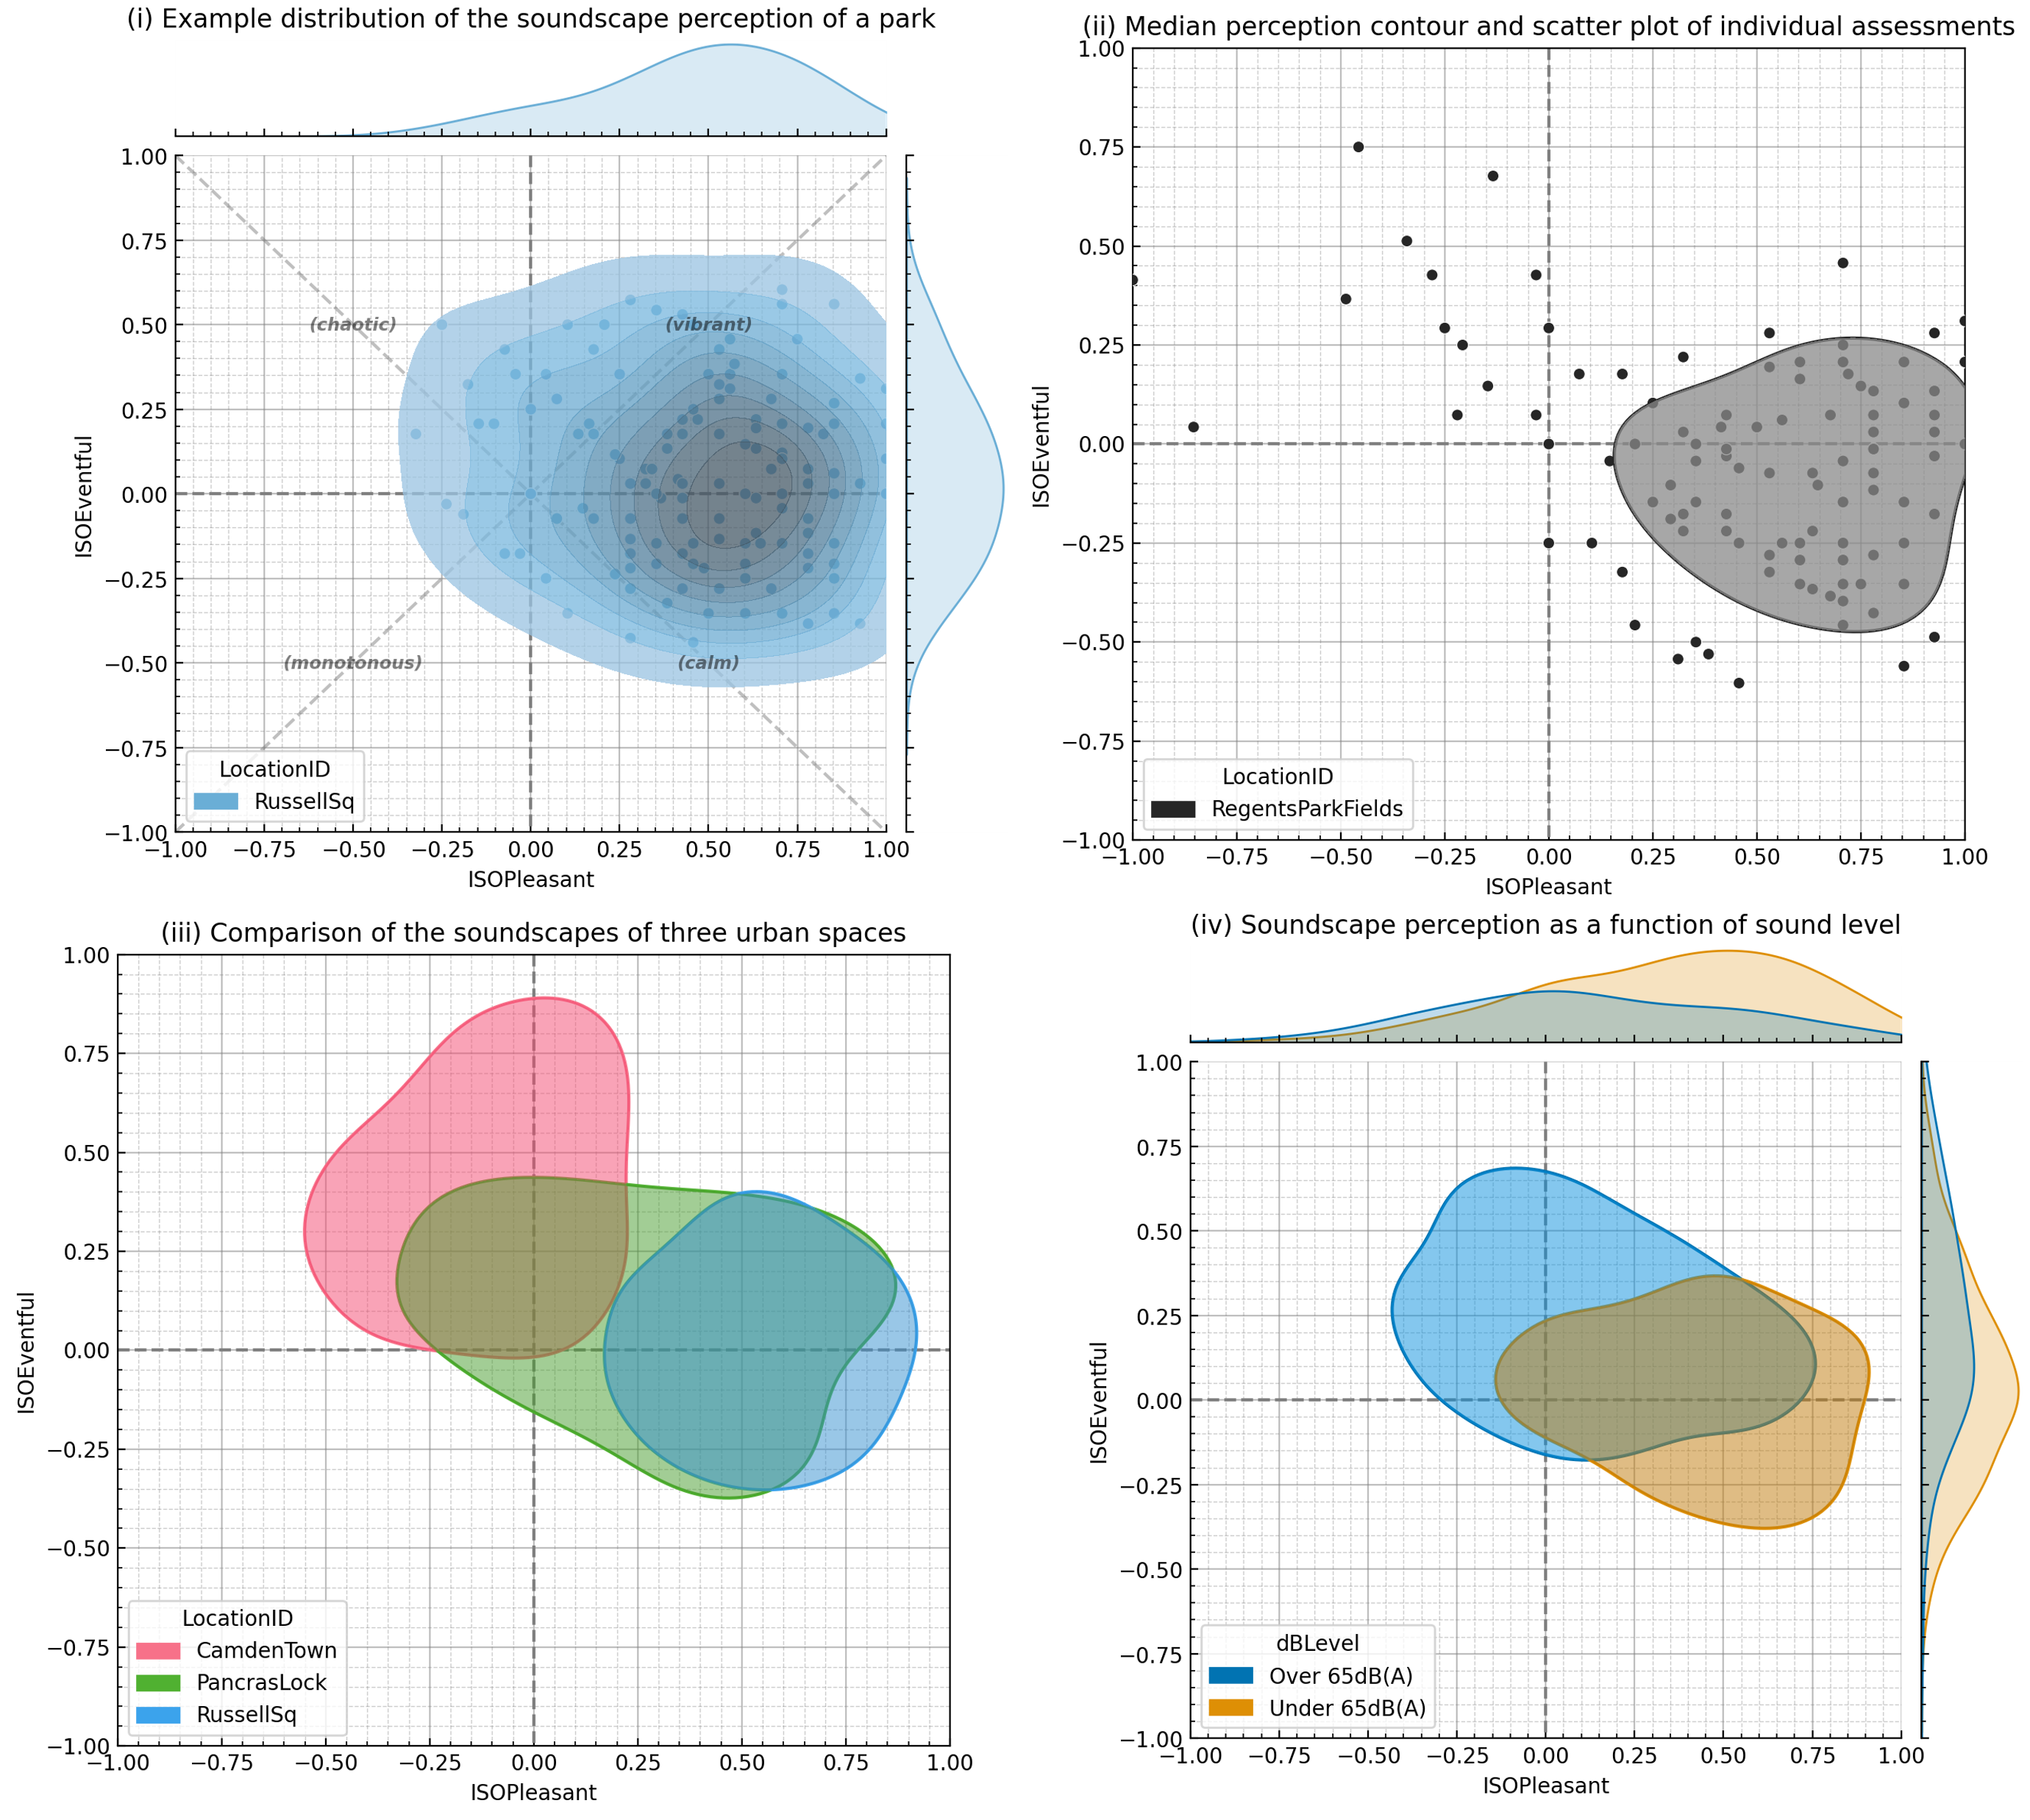
\includegraphics[width=\textwidth]{Figures/jasa-el_Figure2.png}
  \caption{\linespread{1}\selectfont{} A demonstration of some use cases of representing soundscape perception as probabilistic distributions. Data is drawn from the International Soundscape Database (ISD) and is used for demonstration only. (i) Demonstrates a high-level of detail for presenting the bivariate distribution of soundscape perception in a park (Russell Square in London). (ii) Simplified view of the distribution using the \nth{50} percentile contour. The assessments impacted by a series of helicopter fly-overs are made obvious in the chaotic quadrant. (iii) A comparison of three popular public spaces in London. Their overlapping regions can reveal when and how their soundscapes may be similar. (iv) A comparison across the full ISD for soundscape perception at $<65 dB L_{Aeq}$ and $> 65 dBA$. The introduction of other acoustic, environmental, and contextual data can reveal new and complex relationships with the soundscape perception. \label{fig:circ}}
\end{figure}

Once these individual responses are plotted, we then overlay a heatmap of the bivariate distribution (with isodensity curves for each decile) and marginal distribution plots. In this way, three primary characteristics of the soundscape perception can be seen:

\begin{enumerate}
  \item The distribution across both pleasantness and eventfulness, including the central tendency, the dispersion, and any skewness in the response;
  \item The general shape of the soundscape within the space - in this case Russell Square is almost entirely in the pleasant half, but is split relatively evenly across the eventfulness space, meaning while it is perceived as generally pleasant, it is not strongly calm or vibrant;
  \item The degree of agreement about the soundscape perception among the sample - there appears to be a relatively high agreement about the character of Russell Square, as demonstrated by the compactness of the distribution, but this is not the case for every location.
\end{enumerate}

\cref{fig:circ}(a) includes several in-depth visualisations of the distribution of soundscape assessments, however the detail included can make further analysis difficult. In particular, a decile heatmap is so visually busy that, in my experience, it is not possible to plot more than one soundscape distribution at a time without the figure becoming overly busy. It also can make it difficult to truly grasp point 2, the general shape of the soundscape. To facilitate this, the soundscape can be represented by its \nth{50} percentile contour, as demonstrated in \cref{fig:circ}(b) where the shaded portion contains 50\% of the responses. This simplified view of the distribution presents several advantages, as is demonstrated in \cref{fig:circ}(c) and \cref{fig:circ}(d) and takes inspiration from the recommendation in the ISO standard to use the median as a summary statistic. In my testing, the \nth{50} percentile contour has proved useful, clear, and compact, however this should not be taken as the definitive correct percentile cutoff. Further work will need to be done to validate the precise presentation.

When visualised this way, it is possible to identify outliers and responses which are the result of anomalous sound events. For instance if, during a survey session at a calm park, a fleet of helicopters flies overhead, driving the participants to respond that the soundscape is highly chaotic, we would see a group of scatter points in the chaotic quadrant which appear obviously outside the general pattern of responses. Often, these responses would be entirely discarded as outliers or the surveys and soundwalks would be halted entirely -- ignoring what is in fact a significant impact on that location, its soundscape, and how useful it may be for the community. Alternatively, they would be naively included within the statistical analysis, significantly impacting the central tendency and dispersion metrics (i.e. median and range) without consideration for the context. This is the situation shown in \cref{fig:circ}(b) where it is obvious that there is strong agreement that Regents Park Fields is highly pleasant and calm, however we can see numerous responses which assessed it as highly chaotic. These responses were taken when a series of military helicopter fly overs drastically changed the sound environment of the space for several minutes.

\cref{fig:circ}(c) demonstrates how this simplified \nth{50} percentile contour representation makes it possible to compare the soundscape of several locations in a sophisticated way. The soundscape assessments of three urban spaces, Camden Town, Pancras Lock, and Russell Square, are shown overlaid with each other. We can see that Camden Town, a busy and crowded street corner with high levels of traffic noise and amplified music, is generally perceived as chaotic, but the median contour shape which characterises it also crosses over into the vibrant quadrant. We can also see that, for a part of the sample, Russell Square and Pancras Lock are both perceived as similarly pleasant, however some portion of the responses perceived Pancras Lock as being somewhat chaotic and annoying. This kind of visualisation is able to highlight these similarities between the soundscapes in the locations and identify how they differ. From here, further investigation could lead us to answer what factors led to those people perceiving the location as unpleasant, and what similarities the soundscape of Pancras Lock has with Russell Square that could perhaps be enhanced to increase the proportion of people perceiving it as more pleasant.

In addition to solely analysing the distributions of the perceptual responses themselves, this method can also be combined with other acoustic, environmental, and contextual data. The final example, in \cref{fig:circ}(d) demonstrates how this method can better demonstrate the complex relationships between acoustic features of the sound environment and the soundscape perception. The data in the ISD includes approx. 30-s-long binaural audio recordings taken while each participant was responding to the soundscape survey, providing an indication of the exact sound environment they were exposed to. For \cref{fig:circ}(d) the entire dataset of 1,338 responses at all 13 locations has been split according to the analysis of these recordings giving a set of less than 63 dB $L_{Aeq}$ and a set of more than 63 dB. The bivariate distribution of these two conditions are then plotted.

By presenting soundscape perception as a bivariate distributional shape on the circumplex, practitioners are obligated to address two key aspects of perception that are too often ignored: the distribution of potential responses and the eventful dimension. The array of potential responses to an environment is a crucial factor in assessing the successful design of a space and represents the reality of perception. There is no single perceptual outcome of an environment; it will always include some randomness inherent in human perception and this should be reflected in how we present soundscape assessments. Similarly, the eventful dimension is crucial to understanding how an environment is perceived and can have important impacts on the health and well-being of the users. Recent evidence also suggests that there is a more direct relationship between acoustic characteristics and the perception of eventfulness, while pleasantness is more dependent on context \citep{Mitchell2021Investigating}. Studies which explore the correlations between acoustic features and annoyance (or pleasantness) without considering eventfulness are perhaps missing the most direct effect of the acoustic features.

A python package called \texttt{Soundscapy} has been developed for performing the analysis and visualisations presented [making use of the \texttt{seaborn} plotting library \citep{Waskom2021seaborn}] and is available for download from Github \url{(https://github.com/MitchellAcoustics/Soundscapy}. An interactive Jupyter notebook which provides a tutorial for using \texttt{Soundscapy}, working with the \gls{isd} data, and recreating these figures has also been included in the examples folder of the Github repository.

\subsection{A sidenote on the proper distribution for the soundscape circumplex}

The plots shown above make use of a kernel density estimation \citep{Silverman2018} and assumes a normal distribution. Given that the \gls{isopl} and \gls{isoev} values have a hard boundary at $[-1, +1]$, it is not in fact correct to consider the distribution of responses within the circumplex as a normal distribution. A normal distribution is defined as extending out to $(-\infty, \infty)$ with an area of 1 under the probability density. If the potential space of the responses is bounded, the assumption of them forming a normal distribution is violated, as part of the probability density function is unreachable, meaning the area under the probability density will not sum to 1.

If we assume the general shape of the responses to be normal, then they would instead form a truncated normal distribution \citep{Burkardt2014truncated,Barr1999Mean}. Briefly, a truncated normal distribution is estimated by first calculating the probability density function of the standard normal distribution. Then, the density function is truncated at the set boundary ($[a, \infty)$ or $(-\infty, b]$) or boundaries ($[a, b]$) and the portion of the density function which is truncated is redistributed within the boundary.

This redistribution means that the various parameters of a truncated distribution will be somewhat different than for a normal distribution, in particular the calculation of variance. This impacts the soundscape distribution plots demonstrated in \cref{fig:circ} as the kernel density estimation performed by the underlying plotting library (\texttt{seaborn}) assumes a normal distribution with no boundary. It is possible that making use of a truncated normal distribution would change the shape of the distributions produced by \texttt{soundscapy}. Although at this point there does not seem to be a simple method of adapting the \texttt{soundscapy} code to make use of a truncated distribution, I chose to briefly test out how much of a change the truncated distribution is likely to make to the shape of the \texttt{soundscapy} plots through functions available in \texttt{R}.

\begin{figure}[h]
  \centering
  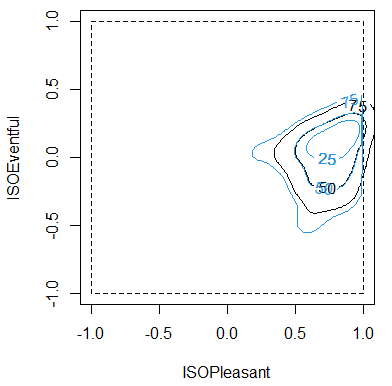
\includegraphics{Figures/Trunc-Normal-demo.png}
  \caption{Comparing a probability distribution in the soundscape circumplex (using Regents Park Japan as the worst case example) using a normal kernel density estimation method (black line) and a truncated KDE (blue line). \label{fig:truncatekde}}
\end{figure}

From \cref{fig:truncatekde}, it appears that there would be some difference in the shape of the soundscape distribution when using a truncated distribution. However, I would note that Regents Park Japan was chosen as the worst case location in the whole \gls{isd} as the samples lie closest to the boundary and the density function estimated in \texttt{soundscapy} has the most area which lies outside the boundary. Most locations do not show any overlap with the boundary and would not be noticeably affected by the truncation. In addition, switching to the truncated normal distribution only affects those iso-density levels which overlap with the boundary. Therefore, the recommended simplified density curve given in \cref{fig:circ}(b) of 50\% is effectively unchanged since it is very unlikely the \nth{50} percentile curve would exceed the boundaries. For the time-being, therefore it appears that there is not a detriment to using a standard normal distribution as opposed to a truncated normal distribution, for the visualisations created by \texttt{soundscapy}.

However, as we move towards a probabilistic prediction framework, and even in the frequentist predictive models used throughout this thesis, it seems possible that the distinctions between these underlying distributions will become more important.

\section{Making Use of the Soundscape Circumplex}
There are various potential methods for integrating the probabilistic soundscape approach into a design and intervention setting. Representing the soundscape as a shape within the circumplex provides flexibility in setting design goals for a space. Not all spaces can or should have the same soundscape and soundscapes should be treated as dynamic, not static; identifying and creating an appropriate soundscape for the particular use case of a space is crucial to guiding its design. Proper forward-looking design of a soundscape would involve defining the desired shape and distribution of perceptions in the space. This can be achieved by drawing the desired shape in the circumplex and testing interventions which will bring the existing soundscape closer to the desired perception. A soundscape may need to be perceived as vibrant during the day and calm for some portion of the evening, meaning the desired shape should primarily sit within the vibrant quadrant but have some overlap into calm. This also enables designers to recognise the limitations of their environment and acknowledge that it is not always possible to transform a highly chaotic soundscape into a calm one. In these cases, instead the focus should be placed on shifting the distribution to some degree in a positive direction. The most sophisticated method of setting design goals is therefore to identify the desired shape which represents the variety of desired outcomes, and focus on designs and interventions which are most successful in matching the predicted outcome with that goal. This strategy of defining the optimal soundscape as an area or a shape within the 2-dimensional circumplex was previously illustrated by \citet{Cain2013development}. In \cref{fig:cainCircumplex}, I have adapted Cain's Figure 6 to show how the shape of a target soundscape can be drawn and the shape of the existing soundscape compared to it. The work of a designer is then trialling intervention options which move the design soundscape closer to the target soundscape. 

\begin{figure}[h]
  \centering
  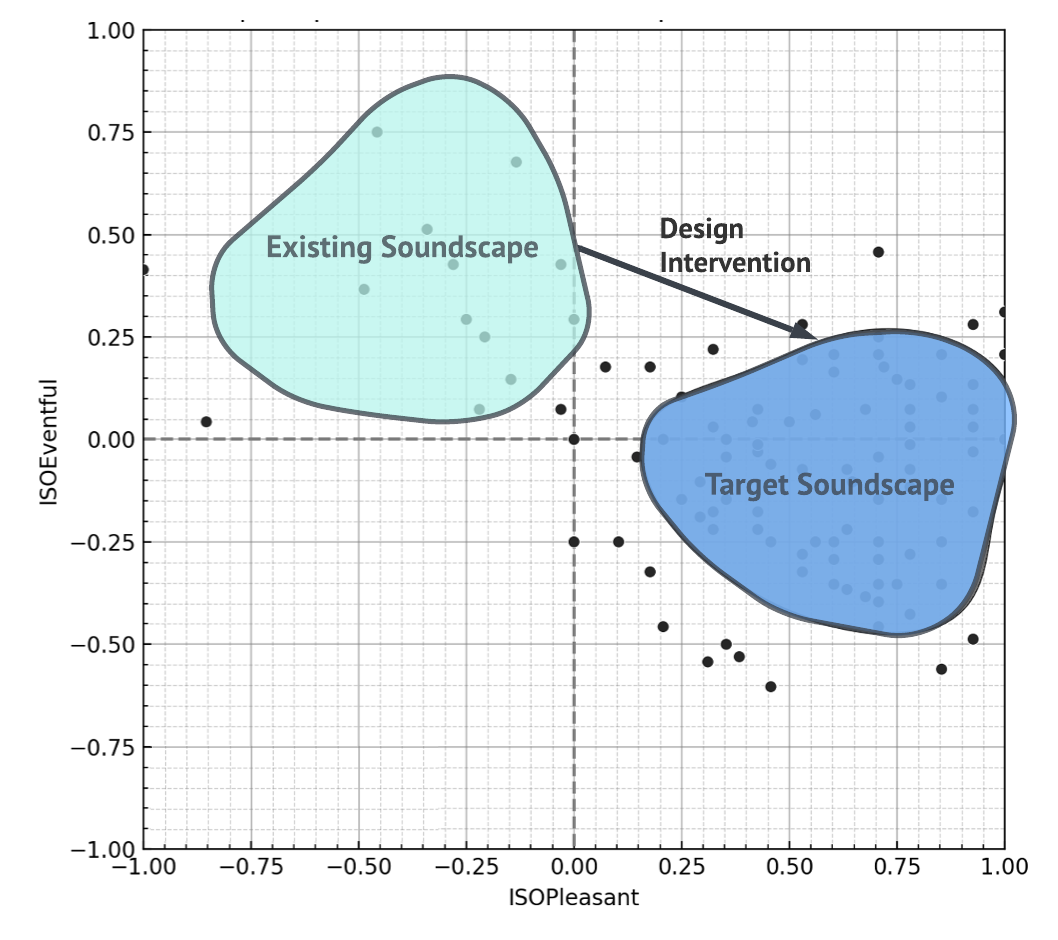
\includegraphics[width=.8\textwidth]{Figures/CainCircumplexTarget.png}
  \caption{Adapted from \citet[Fig. 6]{Cain2013development}. Using the soundscape circumplex shape for target-setting for soundscape design. \label{fig:cainCircumplex}}
\end{figure}

Although the visualisations shown in \cref{fig:circ} are a powerful tool for viewing, analysing, and discussing the multi-dimensional aspects of soundscape perception, there are certainly cases where simpler metrics are needed to aid discussion and to set design goals. Taking inspiration from noise annoyance \citep{ISO15666}, I propose a move toward discussing the `percent of people likely to perceive' a soundscape as pleasant, vibrant, etc. when it is necessary to use numerical descriptions. In this way, a numerical design goal could also be set as e.g. `the soundscape should be likely to be perceived as pleasant by at least 75\% of users' or the result of an intervention presented as e.g. `the likelihood of the soundscape being perceived as calm increased from 30\% to 55\%'. These numbers can be drawn from either actual surveys or from the results of predictive models.

Finally, although acknowledging the distribution of responses is crucial, it is sometimes necessary to summarise locations down to a single point to compare many different locations and to easily investigate how the soundscape assessment has generally changed over time. For this purpose, the mean of the ISOPleasant and ISOEventful values across all respondents is calculated to result in a single coordinate point per location. This clearly mirrors the original intent of the coordinate transformation presented in the ISO, but by applying the transformation first to each individual assessment then calculating the mean value, it maintains a direct link to the distributions shown in \cref{fig:circ}. An example plot using the mean response of each location to compare many locations and to demonstrate change in soundscape perception can be found in \cref{fig:circumplex-locations} \citep[Fig. 5]{Mitchell2021Investigating}. The key to all of these analysis methods, whether they be the distributional plots shown in \cref{fig:circ}, the numerical summaries, or the use of other standard statistical analyses is treating the soundscape of the space or group as a collective perception as expressed by a vector of individual circumplex coordinates.

Finally, the primary concern addressed by this method is the analysis of larger soundscape datasets, compared to what is suggested in the standard. This is necessary in order to statistically describe the groups or sub-groups being investigated, and is typically taken to need a minimum of 30 responses per group (although the full dataset, made up of many groups and locations may have many more responses in total, as in the \gls{isd}) [e.g. \citep{Hong2015Influence,PuyanaRomero2016Modelling}]. It is unlikely that the bivariate distribution plots shown are appropriate for small datasets. However, the process of calculating the ISO coordinates for each individual response and treating this as a set of continuous values to subject to other statistical analyses holds for all sample sizes. Pleasant-eventful scatterplots are still useful for comparing differences in individual responses and appropriate methods of summarising small sample data should be explored (such as the univariate scatterplots described in \citet{Weissgerber2015Bar}).

\subsection{Incorporating appropriateness}

The discussion thus far has focussed on the two primary dimensions of soundscape perception - pleasantness and eventfulness. Our next goal is to somehow account for the third primary component identified by \citet{Axelsson2010principal} - Familiarity, sometimes also referred to as Appropriateness. In a later paper, \citet{Axelsson2015How} addresses critiques of the \gls{ssqp} for its focus on perceptual attributes and its use of a Good-Bad scale, without considering the appropriateness of the soundscape. Given my proposal for representing soundscapes as a shape within the circumplex based on the distribution and for defining a target ideal soundscape shape, we could use additional information about the intended use of the location or the assessed appropriateness of the soundscapes to help identify the best shape for the ideal soundscape. This proposal effectively hinges on the idea that, for a given location and its intended use for relaxation, recreation, or commerce, there is some circumplex shape and placement which would be identified as most appropriate for that context. For a location meant to house an urban market, the most appropriate soundscape would primarily be vibrant, with perhaps some degree of chaotic-ness still being deemed appropriate and perhaps even desirable. For a pocket park meant to provide respite from a busy street, clearly a completely calm soundscape would be preferred, but some degree of monotony could be considered appropriate to the context. In this way, we could make use of appropriateness information to provide a more lenient and achievable definition of the `ideal' distribution of a soundscape, against which the actual soundscape can be assessed. This method could also be further developed to provide a holistic single-value index of soundscape quality by defining standard `ideal' soundscape shapes for different use cases and contexts, with the index indicating to what degree the assessed soundscape conforms to that ideal shape.

\section{Probabilistic Predictions}

This discussion on considering the distribution of responses leads us to my final proposal for improving the general prediction model. The model should be capable of reproducing the current tendency and size of the distribution of responses within the circumplex. This applies both to the prediction for an entire location, with many recordings feeding into the model, but also applies to the results from a single recording. For any single sound or recording, we should acknowledge that there will be a spread of potential responses from the sample population. Even given the exact same inputs, different people will have a range of different responses, all of which should be considered valid. Our goal, therefore, is not only to accurately predict the average response, but also to accurately reflect how much of a spread there will be and how it may be skewed. 

As with many of my proposals for improving our initial model, there are several potential approaches to take -- including a Bayesian approach, as suggested by \citet{Lionello2021Thesis} -- which should be developed as future work in the field. At this stage, I will offer a suggestion based on predicting the standard deviation of responses alongside the average response, which can be combined to generate an outcome distribution\footnote{A version of this was recently done by \citet{Ooi2022Probably} for predicting the probability distribution of \gls{isopl}, however this idea was arrived at independently through the course of writing this chapter.}. The first stage is to perform a deterministic prediction of the ISO coordinates, exactly as in \cref{ch:lockdown}. Then, two additional models will be created for separately predicting the standard deviation of \gls{isopl} and \gls{isoev} responses to a single recording. We would then have four parallel models through which each recording would be processed: one to predict the centre of the \gls{isopl} response, one to predict the standard deviation of the \gls{isopl} response, and the same two for predicting the \gls{isoev} responses. By combining the centre and standard deviation predictions, and assuming a normal (or truncated normal) distribution, we can then generate a probability density function in the two dimensions, resulting in the circumplex shape for that recording. \cref{fig:probPrediction} demonstrates this workflow.

\begin{sidewaysfigure}[h]
  \centering
  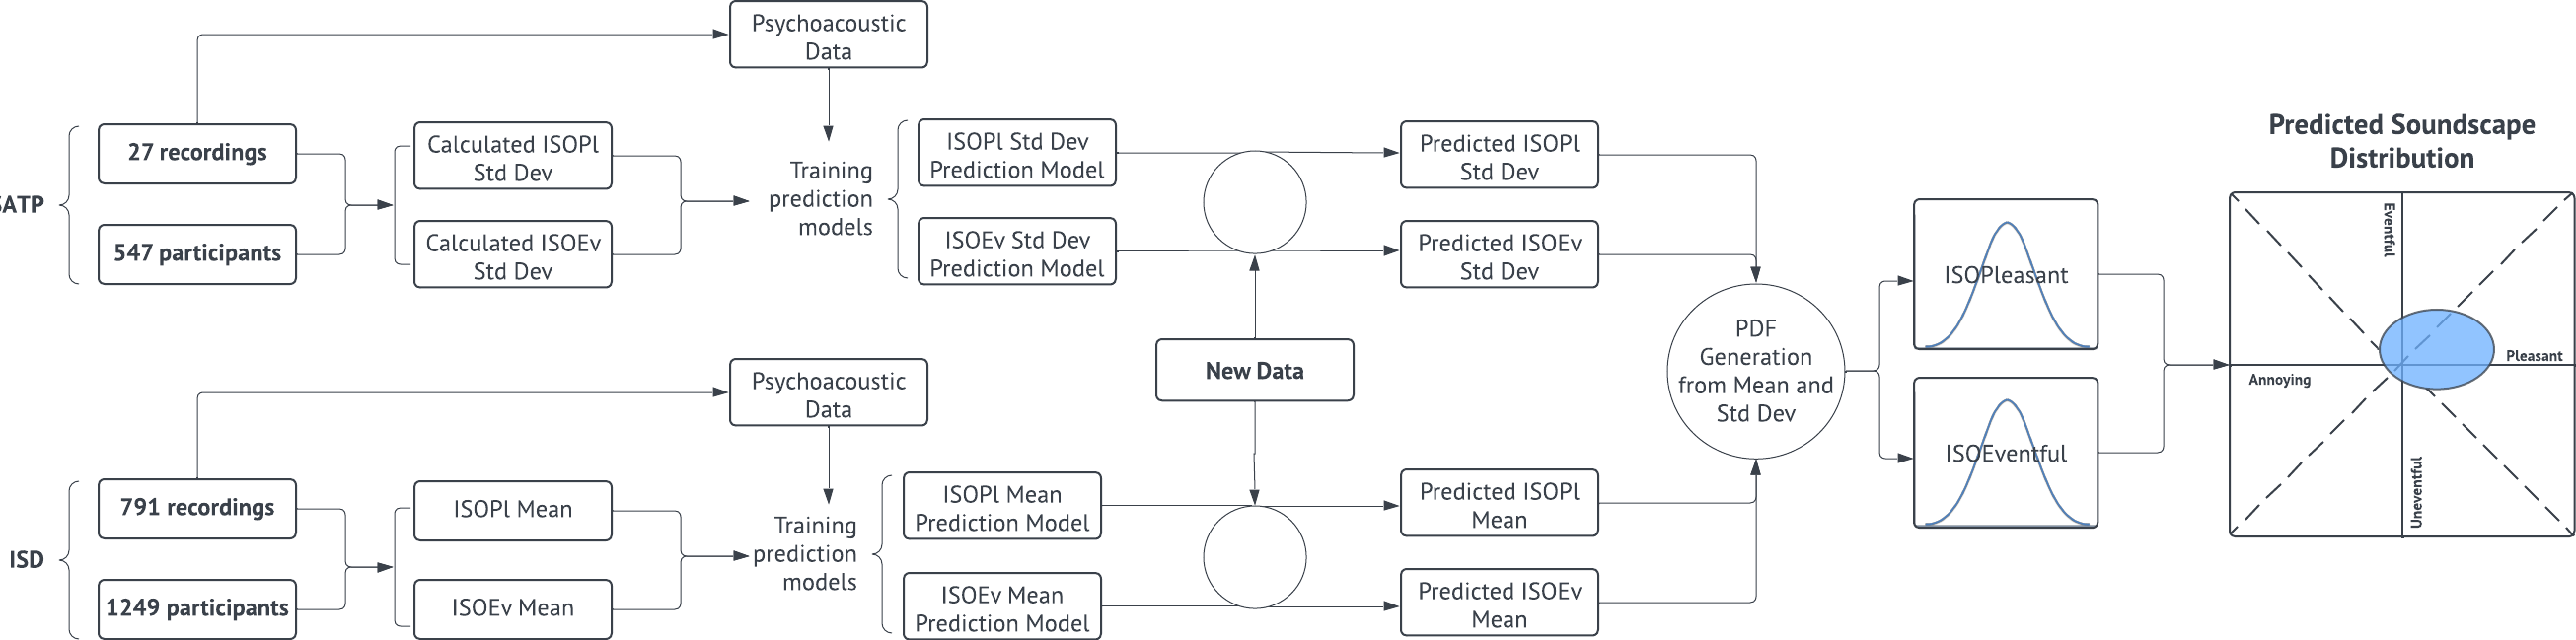
\includegraphics{Figures/Probabilistic Soundscape Prediction.png}
  \caption{\label{fig:probPrediction}}
\end{sidewaysfigure}

In order to train this model, we will need multiple responses per recording in order to calculate the standard deviations for the training set. Some degree of this exists in the \gls{isd}, where we have between an average of 1.57 responses per GroupID, meaning on average 1.57 people conducted their surveys at the same time and thus were exposed to the same sound environment, and indexed to the same binaural recording. However, it seems likely that only 3 responses would not be sufficient to calculate reasonable standard deviation values. In this case, there is a partner dataset to the \gls{isd} which has been created as part of the \glsfirst{satp} \citep{Aletta2020Soundscape}. This project aims to create validated translations of the circumplex \glsplural{paq} into as many other languages as possible, such that soundscape assessments can be carried out across the world using a standardised metric. For this dataset, 27 binaural recordings, made using the same method and equipment as the \gls{isd}, were selected. The specific recordings were selected with the aim of providing a representative range of expected urban soundscapes which evenly cover the circumplex space. After a translation of the perceptual attributes was proposed by a partner research group, they conducted a lab experiment with at least 30 participants all listening to the 27 sounds and completing the soundscape questionnaire. At this stage, this dataset contains 16 languages, with 546 participants each responding to the exact same 27 sounds. This dataset, in addition to its intended use for validating the perceptual attribute translations, also provides a rich dataset to investigate to what degree people's soundscape perception varies in response to the same soundscape, both across the entire dataset and within each language independently. We could thus use this data to train the models for predicting the standard deviation for each recording, and pair this with the centre predictions trained on the much broader \gls{isd} dataset. By combining these datasets and by predicting the expected distribution of responses we create a much more realistic representation of how a population perceives a given soundscape. 

This model would create distribution predictions for each 30s recording which is input to it. To then predict the soundscape distribution of an entire location, we would make many recordings, preferably over several hours or days, and generate the predicted distribution to each of these recordings. These distributions can then be combined to result in an overall predicted distribution of the soundscape of the location, giving us a predicted soundscape shape.

\section{Limitations of the circumplex and quantitative analysis}
The method presented here is a solution for representing the soundscape of a space, which requires considering the perception of many people, but it is important to note that this is only one (very important) goal of the soundscape approach. Psychological and sociological investigations of people's relationship to their sound environment and the interactions between social contexts and individual perception are a crucial aspect of the field for which this approach would likely not be sufficient \citep{Bild2018Public}. Open-response questions, structured interviews, and mixed-methods studies can provide additional insight into how people experience their environment and should be considered alongside or preceding this focus on how a space is likely to be perceived on a larger scale.

These other approaches are not in opposition to the methods proposed here, but instead further expand our view. The circumplex is a limited view of soundscape perception (this is made obvious by the fact that it excludes the third component, \emph{familiarity}, identified in \citet{Axelsson2010principal}) but it is an exceptionally rich tool for dealing with the two primary aspects of soundscape perception which can readily expand the much more limited view provided by existing noise and annoyance assessment tools. Aspects of the psychological and sociological emphasis can also be integrated into a circumplex-focused approach, as demonstrated in \citet{Erfanian2021Psychological}, where personal factors such as age, gender, and psychological well-being were analysed in terms of how they mediated the ISOPleasant and ISOEventful outcomes.

There has been some discussion regarding the interdependence of the PAs and the strict validity of the 90\textdegree and 45 \textdegree relationships between the attributes \citep{Lionello2021Introducing}. Further work has indicated that the scaling between the attributes may vary, but the underlying relationships hold. It is for this reason that I have taken the coordinate projection as the starting point of this critique. It should also be noted that the particular PA descriptors used in ISO 12913 are intended for outdoor environments and should not be directly applied to indoor spaces. However, a proposed set of descriptors for some indoor environments has been derived which further confirms the validity of the circumplex relationships \citep{Torresin2020Indoor}. The methods proposed here should be directly applicable to indoor spaces by using the comfort/content descriptors as well as to any other translations of soundscape descriptors into other languages \citep{Aletta2020Soundscape} as long as the dimensional relationships of the circumplex are maintained.

\section{Conclusion}
\draft{need to adjust and add more general model discussion}
Soundscape studies have been steadily growing as a research field over the past three decades. Their relevance for the planning and design of urban spaces is now generally acknowledged by both the academic and practitioners' communities. Yet, for their contribution in shaping better environments to be meaningful, it is necessary to agree on common methodological approaches and techniques to analyse and present standardised soundscape data. Therefore, the general goal of this work is to consider some of the questions that may still have been left unanswered by the ISO 12913 series when it comes to optimal ways to analyse and represent soundscape data coming from the ISO standardised protocols. As a result, I propose a method for presenting the results of standardised assessments as a distribution of soundscape perception within the circumplex space. This method provides an opportunity to conduct a nuanced discussion of soundscape perception which considers the variety of individual responses. The tools for generating these circumplex visualisation is made openly available as well. This shift is part of a move towards a more holistic approach to urban noise and to integrating the soundscape approach into urban design and regulations.

%%%%%%%%%%%%%%%%%%%%%%%%%%%%%%%%%%%%%%%%%%%%%%%%%%%%%%%%%%%%%%%%%%%%%%%%%

\draft{======= Random bits to incorporate somewhere =======}
\subsubsection{Sound perception as a chaotic system}

Human perception of sound is a chaotic system. Given small changes in a large number of input conditions, a wide range of outcomes are possible \cit{some chaos theory thing}. The same person, exposed to the same environment, could have very different responses to it depending on their state of mind, the route they took to get to the space, what they ate for breakfast, or even just some inherent randomness in their psychological response. This is further amplified by the innumerable differences between people which it will never be possible to fully capture. This is all the more true when discussing in situ perception, outside the controlled conditions of a laboratory.

However, the wide array of previous literature demonstrates that, when taken as a statistical group, conclusions can be made about the probable soundscape perception and its various causal factors.

\begin{quote}
  It means that in many situations, all we can say about a system's dynamics is of a statistical nature. -Gert van der Hejden
\end{quote}